\documentclass{article}
\usepackage[utf8]{inputenc}
\usepackage{amsmath}
\usepackage{graphicx}
\usepackage{physics}
\begin{document}
\section{Problem 2 within project 1}
We are looking to write a program that defines a vector of x-values, and a function that evaluates the excact solution over these values, the results of which
will be stored in 2 columns, with a fixed amount of decimals, in scientific notation. This data will also be plotted  using a separate script.
\subsection*{excact solution}
we require a function that returns $u(x)$ for an input $x$, such that:
\begin{align}    
    \label{eq:excact_solution}
    u(x) =  1 - (1-e^{-10})x - e^{-10x}
\end{align}
The function "analytic\_sol" is declared as the type double, and so is it's (only) parameter "x" too. the function body evaluates $u(x)$ as shown in \ref{eq:excact_solution}, and returns the
result. Vectors x and u were initialized to contain 101 elements doubles, and x was fully defined by assigning each element within a for-loop, iterating through the elements the elements and
assigning each one a value. (each element is assigned the value of the previous element plus 1/100, starting at 0, such that $x_{i+1} = x_i$). u was defined using a for loop, 
calling "analytic\_sol" with $x_i$ as the input, such that $u_{i} = \text{analytic\_sol}(x_i)$.


\begin{figure}
    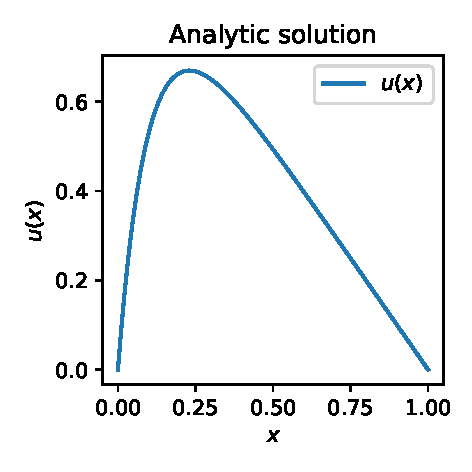
\includegraphics{problem_2_fig.pdf}
    \caption{Shows 101 linearly spaced points starting at 0 and ending at 1, evaluated on the excact solution $u(x)=1 - (1 - e^{-10})x - e^{-10x}$.}
\end{figure}


\end{document}